\section{Additional results}\label{sec:extra_results}


\subsection{Model performance}

Here we present accuracy and loss values for Llama2-7B, Llama2-70B and Gemma3-4B on the five datasets we study.
Results for Llama 2 here match those published in \citet{kossen2024context}.


\begin{table}[h]
    \centering
    \small
    \begin{tabular}{l c c c c c c}
        \toprule
        Dataset & L-7B-zero & L-7B-few & L-70B-zero & L-70B-few & G-4B-zero & G-4B-few\\
        \midrule
        FPB & 66.75 & 90.60 & 26.25 & 94.15 & 29.70 & 91.00\\
        SST-2  & 63.96 & 92.19 & 76.80 & 93.60 & 57.79 & 91.68\\
        Subj & 49.38 & 89.72 & 54.85 & 96.12& 50.40 & 93.73\\
        HS & 11.38 & 89.28 & 84.18 & 90.23 & 42.87 & 89.42\\
        MMLU & 35.41 & 42.16 & 60.80 & 65.34 & 52.61 & 57.83 \\
       \bottomrule
    \end{tabular}
    \vspace{1em}
    \caption{Accuracy (\%) of Llama 2 (L) 7B and 70B models and Gemma3-4B (G) model evaluated on pool sets.}
    \label{tab:accuracy_models}
\end{table}


\begin{table}[h]
    \centering
    \small
    \begin{tabular}{l c c c c c c}
        \toprule
        Dataset & L-7B-zero & L-7B-few & L-70B-zero & L-70B-few & G-4B-zero & G-4B-few\\
        \midrule
        FPB & 0.7847 & 0.3084 & 1.3123 & 0.2152 & 1.4695 & 0.2701\\
        SST-2  & 0.5639 & 0.2050 & 0.5808 & 0.1828 & 0.6234 & 0.2107\\
        Subj & 0.7326 & 0.3278 & 0.5873 & 0.1235&0.7101 & 0.2741\\
        HS & 0.9129 & 0.2979 & 0.5386 & 0.2166 &0.7245 & 0.2678\\
        MMLU & 1.3468 & 1.2568 & 0.9217 & 0.8384 & 1.0920 & 0.9683 \\
        \bottomrule
    \end{tabular}
    \vspace{1em}
    \caption{Loss of Llama 2 (L) 7B and 70B models and Gemma3-4B (G) model evaluated on pool sets.}
    \label{tab:loss_models}
\end{table}


\subsection{Failure mode on Subjectivity}


\begin{table}[t]
    \centering
    \small
    \begin{tabular}{l c c c c}
        \toprule
        Dataset & 70B (T) \& 70B (S) & 70B (T) \& 7B (S) & 7B (T) \& 70B (S) & 7B (T) \& 7B (S) \\
        \midrule
        FPB & 0.628 & 0.392 & 0.707 & 0.588\\
        SST-2 & \textbf{0.285} & 0.224 & 0.527 & 0.454\\
        Subj & 0.364 & \textbf{-- 0.025}& 0.802 & 0.652\\
        HS & 0.461 & 0.146 & 0.555 & 0.384\\
        \bottomrule
    \end{tabular}
    \vspace{1em}
    \caption{
        Pearson's correlation coefficient between the cross-entropy of the surrogate (S) and target (T) models' predictions and the negative log likelihood of the target model's predictions.
        Low or negative correlation indicates poor alignment between surrogate-based acquisition and optimal acquisition.
        Failure cases are in bold.
    }
    \label{tab:pearson_fewshot}
\end{table}


Here we build on our failure analysis in \Cref{sec:failure} (where we investigated why LURE-70B failed for the 70B-few target model on the SST-2 dataset), now focusing on the underperformance of LURE-7B for the 70B-few target model on the Subj dataset.
We find that filtering out high-loss examples does not improve performance like it did in the SST-2 case, but we do find some insight from another line of investigation.
In particular we compute the Pearson correlation coefficient between the cross-entropy-based acquisition scores and the optimal acquisition function (negative log likelihood of the target model's predictions), with this correlation quantifying how well surrogate-based acquisition approximates optimal acquisition.
Notably this is the only setting where the correlation is close to zero and is negative.
This indicates that the surrogate model provides no meaningful guidance, helping to explain why active testing performs similarly to uniform-random testing in this case.


\subsection{Smaller surrogate models on the four core datasets}


\begin{figure}[h]
    \begin{subfigure}[b]{\linewidth}
        \centering
        % trim={<left> <lower> <right> <upper>}
        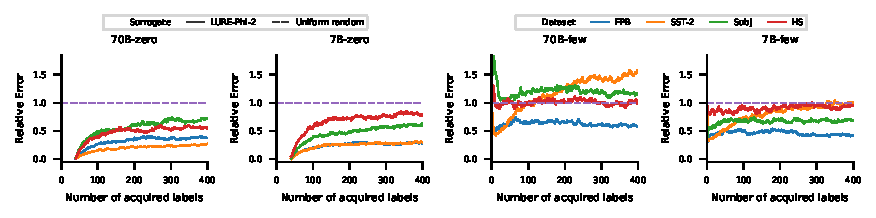
\includegraphics[width=\linewidth,trim={0 5pt 0 0}]{
            figures/pdf/relative_errors_phi2.pdf
        }
        \caption{Llama 2 target models and Phi-2 surrogate model}
         \label{fig:7b_70b_phi_unif_lure}
    \end{subfigure}
    \begin{subfigure}[b]{\linewidth}
        \centering
        % trim={<left> <lower> <right> <upper>}
        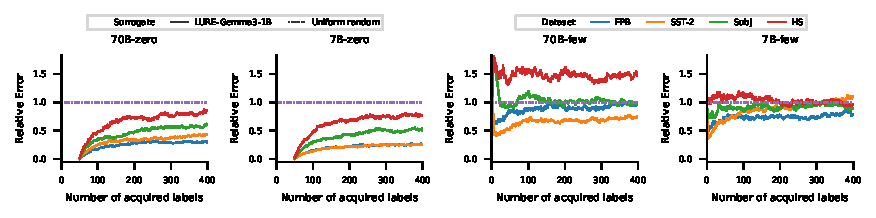
\includegraphics[width=\linewidth,trim={5pt 5pt 0 0}]{
            figures/pdf/relative_errors_gemma_1b.pdf
        }
        \caption{Llama 2 target models and Gemma3-1B surrogate model}
        \label{fig:7b_70b_gemma3_1b_unif_lure}
    \end{subfigure}
    \caption{
        Even very small surrogate models can support effective active testing in simple cases, although they struggle with evaluating our best-performing target model, 70B-few.
    }
    \label{fig:7b_70b_phi_gemma1b}
\end{figure}


Here we explore two surrogate models that are smaller than those used in \Cref{sec:experiments}: Phi-2 2.7B (\citealp{javaheripi2023phi}; MIT License) and Gemma3-1B (\citealp{kamath2025gemma}; Gemma License).
We see both surrogate models producing strong performance in evaluating 70B-zero and 7B-zero, and more mixed performance in evaluating the two stronger target models, 70B-few and 7B-few (\Cref{fig:7b_70b_phi_gemma1b}).


\subsection{Smaller surrogate model on MMLU}\label{section:failure_case_mmlu}


\begin{figure*}[h]
    \centering
    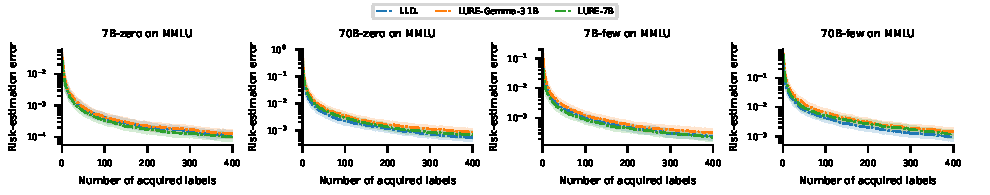
\includegraphics[width=\linewidth]{
        figures/pdf/mmlu_gemma3_1b_errors.pdf
    }
    \caption{
        A sufficiently weak surrogate model can cause active testing to consistently fail on MMLU.
    }
    \label{fig:7b_70b_gemma3_1b_mmlu}
\end{figure*}


Here we revisit Gemma3-1B as a surrogate model, now on the harder MMLU dataset.
We see active testing failing to outperform uniform-random testing (\Cref{fig:7b_70b_gemma3_1b_mmlu}).
This can be explained by how poorly Gemma3-1B performs on MMLU: it achieves approximately 25\% accuracy, the base accuracy produced by uniform-random prediction.
A weak surrogate model can thus undermine active testing.


\subsection{Dynamic-surrogate active testing}\label{sec:dynamic_surrogate}

Here we explore the use of dynamic surrogate models, in contrast with the fixed surrogate models we use in our approach.
In the dynamic approach the surrogate model's context incorporates newly acquired labels, leading to recomputed predictions, and thus novel acquisition probabilities at each sampling step.
Our experiments focus on few-shot Llama2-7B and Llama2-70B target models with dynamic and fixed Llama2-7B surrogate models.
We start with 10 in-context examples and run 40 steps of data acquisition.
We run for 50 random-number seeds for dynamic-surrogate active testing, and for 3,000 seeds for fixed-surrogate active testing and uniform-random active testing.

Despite being much more computationally expensive, dynamic-surrogate active testing shows no consistent improvement in risk estimation over fixed-surrogate active testing (\Cref{tab:dynamic_7b,tab:dynamic_70b}).
Thus, while dynamic surrogate models might be useful elsewhere, the results we see for our selection of datasets support our design choice of fixing the surrogate model: it improves over uniform-random testing while maintaining a low computational cost and thus readily scaling to LLM evaluations.


\begin{table}[h]
    \centering
    \small
    \begin{tabular}{l l c c c c}
        \toprule
        Dataset & Testing method & Step 10 & Step 20 & Step 30 & Step 40 \\
        \midrule
        \multirow{6}{*}{SST-2}& \multirow{2}{*}{Uniform random} & 91.41 &45.49  & 29.25 	& 20.66 \\
        &&(87.04, 95.86)	& (43.53, 47.52)	& (28.00, 30.51)& (19.82, 21.52)\\
        \cline{2-6}
        &\multirow{2}{*}{LURE-7B dynamic} & 63.25  &	22.79 	& 13.52 	&8.62 \\
        &&(36.23, 96.67)&(14.56, 32.91)&(8.93, 18.80)&(5.82, 11.88)\\
        \cline{2-6}
        & \multirow{2}{*}{LURE-7B fixed} & 42.71 	&19.99 	&12.42 	&8.74 \\
        &&(40.32, 45.11)&(19.07, 20.96)&(11.87, 13.00)&(8.38, 9.11)\\
        \cline{1-6}
        \multirow{6}{*}{FPB}& \multirow{2}{*}{Uniform random} & 135.75 &	65.14 &	40.06 &	27.99 \\
        &&(130.00, 141.72)&(62.37, 68.05)&(38.41, 41.76)&(26.84, 29.16)\\
        \cline{2-6}
        & \multirow{2}{*}{LURE-7B dynamic} & 65.73 &	36.40 	&18.33 	&11.53 \\
        &&(45.79, 86.86)&(25.31, 49.18)&(11.82, 25.79)&(7.37, 16.43)\\
        \cline{2-6}
        & \multirow{2}{*}{LURE-7B fixed} & 77.54 	&36.88 	&22.97	&16.26 \\
        &&(73.39, 81.94)&(35.22, 38.61)& (21.99, 23.95)&(15.56, 16.96)\\
        \cline{1-6}
        \multirow{6}{*}{HS}& \multirow{2}{*}{Uniform random} & 156.59 &	96.51  &	77.32 &	66.84 \\
        &&(152.02, 161.10)&(93.78, 99.32)&(75.14, 79.54)&(64.93, 68.76)\\
        \cline{2-6}
        & \multirow{2}{*}{LURE-7B dynamic} & 121.45 	&75.61 	&52.12  &	43.83 \\
        &&(100.99, 142.89)&(60.04, 91.73)&(40.48, 64.84)&(35.35, 52.63)\\
        \cline{2-6}
        & \multirow{2}{*}{LURE-7B fixed} & 144.44  &	89.65  &	72.62  &	63.67 \\
        &&(139.38, 149.87)&(87.31, 91.98)&(70.73, 74.47)&(62.07, 65.31)\\
        \cline{1-6}
        \multirow{6}{*}{Subj}& \multirow{2}{*}{Uniform random} & 46.97 &	21.79 &	13.76 &	10.23 \\
        &&(44.97, 49.00)&(20.89, 22.70)&(13.19, 14.36)&(9.80, 10.66)\\
        \cline{2-6}
        & \multirow{2}{*}{LURE-7B dynamic} & 71.76&	35.25 &	36.75&	30.94 \\
        && (50.93, 95.54)&(20.62, 53.32)& (21.11, 55.19)&(18.43, 46.09)\\
        \cline{2-6}
        & \multirow{2}{*}{LURE-7B fixed} & 40.20 &	19.69 &	12.95 &	9.12 \\
        &&(38.39, 42.02)&(18.89, 20.48)&(12.42, 13.50)&(8.73, 9.52)\\
        \bottomrule
    \end{tabular}
    \vspace{1em}
    \caption{
        Mean squared error (multiplied by $10^4$; mean on first row; 5th and 95th percentile on second row) for uniform-random testing, dynamic-surrogate active testing and fixed-surrogate active testing of 7B-few.
    }
    \label{tab:dynamic_7b}
\end{table}


\begin{table}[h]
    \centering
    \small
    \begin{tabular}{l l c c c c}
        \toprule
        Dataset & Testing method & Step 10 & Step 20 & Step 30 & Step 40 \\
        \midrule
        \multirow{6}{*}{SST-2}& \multirow{2}{*}{Uniform random} & 81.75 &	40.04 &	25.01 &	17.92 \\
        &&(77.77, 85.85) & (38.24, 41.87) & (23.98, 26.06) & (17.19, 18.66) \\
        \cline{2-6}
        & \multirow{2}{*}{LURE-7B dynamic} & 28.76 &	17.21 &	12.62 &	8.57 \\
        &&(22.13, 35.70) &(11.42, 23.89) &(8.83, 16.74) &(6.37, 11.07) \\
        \cline{2-6}
        & \multirow{2}{*}{LURE-7B fixed} & 40.09&	19.11 &	12.26&	8.44 \\
        && (38.28, 41.98) &(18.35, 19.89) & (11.80, 12.73) &(8.12, 8.76) \\
        \cline{1-6}
        \multirow{6}{*}{FPB}& \multirow{2}{*}{Uniform random} & 173.90 &	80.36 &	50.14 &	35.07 \\
        &&(164.57, 183.50) &(76.55, 84.22) &(47.77, 52.54) &(33.40, 36.83) \\
        \cline{2-6}
        & \multirow{2}{*}{LURE-7B dynamic} & 114.11 &	34.89 &	19.71 &	11.10 \\
        &&(84.88, 144.11) &(25.00, 46.22) &(13.20, 27.05) &(7.68, 14.95) \\
        \cline{2-6}
        & \multirow{2}{*}{LURE-7B fixed} & 150.45 &	70.59 &	45.85 &	33.25 \\
        &&(140.12, 161.06) &(66.56, 74.69) &(43.59, 48.21) &(31.64, 34.85) \\
        \cline{1-6}
        \multirow{6}{*}{HS}& \multirow{2}{*}{Uniform random} & 98.22 &	48.73 &	33.04 &	25.27 \\
        &&(94.33, 102.28) & (46.95, 50.54) &(31.84, 34.29) &(24.36, 26.20) \\
        \cline{2-6}
        & \multirow{2}{*}{LURE-7B dynamic} & 88.73 &	41.15 &	23.93 &	16.18 \\
        &&(64.35, 116.85) &(31.37, 51.26) &(18.57, 29.54) &(12.40, 20.03) \\
        \cline{2-6}
        & \multirow{2}{*}{LURE-7B fixed} & 74.57 &	39.31 &	26.87 &	19.93 \\
        &&(71.50, 77.75) &(37.78, 40.87) &(25.85, 27.89) &(19.18, 20.69) \\
        \cline{1-6}
        \multirow{6}{*}{Subj}& \multirow{2}{*}{Uniform random} & 109.53 &	66.96 &	51.41 &	42.97 \\
        &&(105.47, 113.54) &(64.75, 69.11) &(49.77, 53.10) &(41.59, 44.36) \\
        \cline{2-6}
        & \multirow{2}{*}{LURE-7B dynamic} & 209.81 &	134.48 &	72.61 &	64.43 \\
        &&(161.39, 260.62) &(99.07, 172.06) &(54.29, 92.06) &(48.04, 82.24) \\
        \cline{2-6}
        & \multirow{2}{*}{LURE-7B fixed} & 134.87 &	77.31 &	57.14 &	47.24 \\
        &&(129.79, 140.22) &(74.56, 80.06) &(55.20, 59.07) &(45.64, 48.81) \\
        \bottomrule
    \end{tabular}
    \vspace{1em}
    \caption{
        Mean squared error (multiplied by $10^4$; mean on first row; 5th and 95th percentile on second row) for uniform-random testing, dynamic-surrogate active testing and fixed-surrogate active testing of 70B-few.
    }
    \label{tab:dynamic_70b}
\end{table}


\clearpage

\subsection{Risk-estimation values}

In addition to the plots shown in \Cref{sec:experiments}, we present numerical values for the risk-estimation error of uniform-random testing and active testing (with the cross-entropy acquisition function) at acquisition steps 50, 100, 200, 300 and 400 in \Cref{tab:1,tab:2,tab:3,tab:4,tab:5}.


\begin{table}[h]
    \centering
    \small
    \begin{tabular}{l l c c c c c}
        \toprule
        Target model & Testing method & Step 50 & Step 100 & Step 200 & Step 300 & Step 400 \\
        \midrule
        \multirow{4}{*}{70B-zero} & Uniform random & 24.3373 & 11.5663 & 5.1944 & 3.4854 &2.4122\\
        &LURE-Llama2-7B & --- & 8.0511 & 3.6772  & 1.7589  & 1.0463 \\
        &LURE-Llama2-70B & --- & \textbf{4.2225} & \textbf{2.0045}  & \textbf{0.98390}  & \textbf{0.64870} \\
        &LURE-Gemma3-4B & --- & 7.1132 & 3.5176 & 1.6571 & 1.0540 \\
        \hline
        \multirow{4}{*}{7B-zero}& Uniform random & 9.4687   & 4.8302 &  2.1823 &  1.4524 &  1.0075\\
        & LURE-Llama2-7B & --- & 2.5167  &  1.3094  &  0.59430 &  0.37380 \\
        & LURE-Llama2-70B & --- & 1.9294  &  0.96850 & 0.42460 & 0.27060 \\
        &LURE-Gemma3-4B & --- & \textbf{1.1421} &\textbf{0.5849}& \textbf{0.3681}&
        \textbf{0.2341}\\
        \hline
        \multirow{4}{*}{70B-few}&  Uniform random & 10.5749 &  5.16310  &  2.48680  & 1.51150  &  0.977800 \\
        &LURE-Llama2-7B & 6.3984  &  3.2058  &  1.3719  &  0.89110 &  0.63880 \\
        & LURE-Llama2-70B & 5.0757 &  \textbf{2.5057}   & \textbf{1.1921}   & \textbf{0.76740}  & \textbf{0.54300} \\
        &LURE-Gemma3-4B & \textbf{5.0390} &  2.6267& 1.3102& 0.8344&
        0.5825\\
        \hline
        \multirow{4}{*}{7B-few} & Uniform random &14.3272 &  7.2276& 3.4608 &  2.3147 & 1.5246 \\
        & LURE-Llama2-7B & 8.9252 &  4.5853 &  2.3314 &  1.5486 &  1.1345 \\
        & LURE-Llama2-70B & \textbf{4.8174 } &  \textbf{2.1675}  &  \textbf{1.1186 } &  \textbf{0.65290}  & \textbf{ 0.45770} \\
        &LURE-Gemma3-4B & 6.5254 & 3.7684 &1.9489& 1.2371& 0.8556 \\
        \bottomrule
    \end{tabular}
    \vspace{1em}
    \caption{
        Risk-estimation error (multiplied by $10^4$; minimum per target model in bold) for the FPB dataset.
    }
    \label{tab:1}
\end{table}


\begin{table}[h]
    \centering
    \small
    \begin{tabular}{l l c c c c c}
        \toprule
        Target model & Testing method & Step 50 & Step 100 & Step 200 & Step 300 & Step 400 \\
        \midrule
        \multirow{4}{*}{70B-zero}& Uniform random & 2.1154 &  1.0992 &  0.56060 &  0.34910  & 0.26150 \\
        & LURE-Llama2-7B & --- & 0.5386 &  0.3089 &  0.1551 &  0.1023  \\
        & LURE-Llama2-70B & --- & \textbf{0.4191}  & \textbf{0.2308} &  \textbf{0.1255 } & \textbf{0.08190} \\
        & LURE-Gemma3-4B & --- & 0.5283& 0.2790 & 0.1542& 0.1042 \\
        \hline
        \multirow{4}{*}{7B-zero}& Uniform random &12.4455&  5.49 &   2.9545&  1.9694&  1.362 \\
        & LURE-Llama2-7B & --- & 2.7160  & 1.4229 &  0.66190 &  0.48410 \\
        & LURE-Llama2-70B & --- & \textbf{2.3740}  & \textbf{1.2437}  & \textbf{0.60510}  & \textbf{0.42530 } \\
        &LURE-Gemma3-4B & --- & 3.5371 & 1.6843& 0.8699& 0.6062\\
        \hline
        \multirow{4}{*}{70B-few}& Uniform random & 36.6017& 16.8825 &9.4717&  6.3474&  4.3089 \\
        &LURE-Llama2-7B  & \textbf{24.8052}&  \textbf{14.7678}&   \textbf{7.9162} & \textbf{5.2615} & \textbf{4.0596} \\
        & LURE-Llama2-70B  & 40.8407&  30.077 &  21.3892 & 17.1808 & 14.7939 \\
        &LURE-Gemma3-4B & 26.3377& 16.8812& 9.4499& 7.1826 & 5.7175\\
        \hline
        \multirow{4}{*}{7B-few}& Uniform random & 19.5177&  9.5602 & 4.9347&  3.1286 & 2.2497 \\
        &LURE-Llama2-7B &14.2747&  8.3696&  4.6265&  3.2263 & 2.3764 \\
        &LURE-Llama2-70B & \textbf{9.7216}&  \textbf{6.4914} & \textbf{3.6886}& 2.8971&  2.1722 \\
        &LURE-Gemma3-4B & 13.3504& 7.0426& 3.9896& \textbf{2.8028}&\textbf{1.9958}\\
        \bottomrule
    \end{tabular}
    \vspace{1em}
    \caption{
        Risk-estimation error (multiplied by $10^4$; minimum per target model in bold) for the SST-2 dataset.
    }
    \label{tab:2}
\end{table}


\begin{table}[h]
    \centering
    \small
    \begin{tabular}{l l c c c c c}
        \toprule
        Target model & Testing method & Step 50 & Step 100 & Step 200 & Step 300 & Step 400 \\
        \midrule
        \multirow{4}{*}{70B-zero}& Uniform random & 1.2104    &  0.64740    &  0.30890    &  0.21120    &  0.15430 \\
        &LURE-Llama2-7B & --- & 0.4688   & 0.2311   &  0.1113   &   0.07570 \\
        & LURE-Llama2-70B & --- & \textbf{0.139  } &  \textbf{0.0758}   & \textbf{0.0373 }  &  \textbf{0.0251} \\
        &LURE-Gemma3-4B & --- & 0.3809& 0.1897& 0.0887& 0.0638\\
        \hline
        \multirow{4}{*}{7B-zero}& Uniform random& 9.7212 &  5.1028& 2.4378 &  1.5612 &  1.1429 \\
        & LURE-Llama2-7B & --- & 3.4150  &  1.6835   & 0.87130   & 0.58730 \\
        &LURE-Llama2-70B &--- &\textbf{1.6958 } &  \textbf{0.89970 } & \textbf{ 0.44150}  &  \textbf{0.29280} \\
        &LURE-Gemma3-4B & --- & 2.8896& 1.4536& 0.7144& 0.4787\\
        \hline
        \multirow{4}{*}{70B-few}& Uniform random & 15.5609 &  6.6315  & 3.7465 &  2.5614 &  2.1347 \\
        & LURE-Llama2-7B &16.4075 &  8.2611 &  4.4942 &  3.1802 &  2.1987 \\
        & LURE-Llama2-70B & \textbf{8.2473 } &  \textbf{5.0366} &   \textbf{3.0052} &  \textbf{ 2.1589} &  \textbf{ 1.6293} \\
        &LURE-Gemma3-4B & 12.615 & 6.7789& 3.3058& 2.2544 & 1.7645\\
        \hline
        \multirow{4}{*}{7B-few}&Uniform random & 7.4461   & 3.9287   & 1.8132  &  1.1308   & 0.87000 \\
        & LURE-Llama2-7B &5.2522   & 2.6268  &  1.2944   & 0.84500   & 0.63670 \\
        & LURE-Llama2-70B & \textbf{1.8539}   & \textbf{1.0921}  &  \textbf{0.62250 } &  \textbf{0.42070}  &  \textbf{0.30200} \\
        &LURE-Gemma3-4B & 4.1246& 2.1545& 1.0256& 0.6868 & 0.4941\\
        \hline
    \end{tabular}
    \vspace{1em}
    \caption{
        Risk-estimation error (multiplied by $10^4$; minimum per target model in bold) for the Subj dataset.
    }
    \label{tab:3}
\end{table}


\begin{table}[h]
    \centering
    \small
    \begin{tabular}{l l c c c c c}
        \toprule
        Target model & Testing method & Step 50 & Step 100 & Step 200 & Step 300 & Step 400 \\
        \midrule
        \multirow{4}{*}{70B-zero}& Uniform random & 2.3826  &  1.1493  &  6.3630  &  0.39690   & 0.30590 \\
        &LURE-Llama2-7B& --- & 0.8497   & 0.4371   & 0.2247  &  0.1524 \\
        &LURE-Llama2-70B & --- & \textbf{0.5703 }  & \textbf{0.2996}  & \textbf{ 0.1418 } & \textbf{ 0.09900 } \\
        &LURE-Gemma3-4B & --- & 0.7508& 0.3700& 0.1822& 0.1330\\
        \hline
        \multirow{4}{*}{7B-zero}& Uniform random& 4.3455  &  \textbf{2.3304}   & \textbf{1.3545}  &  0.96420  &  0.80470 \\
        & LURE-Llama2-7B & --- &3.8653  & 1.9395  &  1.1326  &  0.86310 \\
        & LURE-Llama2-70B &---& 3.0157  & {1.7693}  &  \textbf{0.94190}  & \textbf{ 0.73000} \\
        &LURE-Gemma3-4B & --- & 3.5508& 1.6981& 0.9918& 0.7766\\
        \hline
        \multirow{4}{*}{70B-few}& Uniform random & 24.5497 &  11.8593  &  5.8947 &   4.263 &    2.897 \\
        &LURE-Llama2-7B &  26.4253 &  13.5746 &   6.9755 &   4.249  &   3.0014 \\
        & LURE-Llama2-70B &  19.8693  & 11.2704  &  6.1626 &   \textbf{3.983} &    2.9785 \\
        &LURE-Gemma3-4B & \textbf{19.4658}& \textbf{10.4853}& \textbf{5.473}& \textbf{3.6247} & \textbf{2.767}\\
        \hline
        \multirow{4}{*}{7B-few}& Uniform random & 23.7706  & 11.7404  &  6.6989  &  4.6215 &   3.4943 \\
        &LURE-Llama2-7B &19.6371 &   9.638 &    5.8037 &   4.0226 &3.1452 \\
        &LURE-Llama2-70B & \textbf{13.4897} &   \textbf{7.5196} &   \textbf{4.1388}  &  \textbf{2.7654}&  \textbf{2.2691} \\  
        &LURE-Gemma3-4B & 16.6135& 8.7585& 4.8131& 3.4505 & 2.8044\\
        \hline      
    \end{tabular}
    \vspace{1em}
    \caption{
        Risk-estimation error (multiplied by $10^4$; minimum per target model in bold) for the HS dataset.
    }
    \label{tab:4}
\end{table}


\begin{table}[h]
    \centering
    \small
    \begin{tabular}{l l c c c c c}
        \toprule
        Target model & Testing method & Step 50 & Step 100 & Step 200 & Step 300 & Step 400 \\
        \midrule
        \multirow{3}{*}{70B-zero}& Uniform random & 45.2305 & 22.0405& 11.5532& 7.2541& 5.288 \\
        &LURE-Llama2-7B  & 57.137 & 28.4008& 13.3008& 8.4398&6.7655 \\
        &LURE-Llama2-70B &\textbf{30.4079}& {17.3273}& {9.5205}& {6.6253}& 4.9939 \\
        & LURE-Gemma3-4B & 30.894 & \textbf{16.3988}& \textbf{9.0229}& \textbf{5.6838}& \textbf{4.1935} \\
        \hline
        \multirow{4}{*}{7B-zero}& Uniform random& 8.1557& 4.1386& 2.1924& 1.4752& 1.1799 \\
        & LURE-Llama2-7B  & 6.6835& 3.2991& 1.6763& 1.2791&0.9767 \\
        & LURE-Llama2-70B &\textbf{4.3678}& \textbf{2.6164}& \textbf{1.3063}& \textbf{0.9088}&\textbf{0.7330} \\
        &LURE-Gemma3-4B & 4.9507& 2.6543& 1.4700& 0.9569 &0.7622 \\
        \hline
        \multirow{4}{*}{70B-few}& Uniform random & {80.9096}& {41.8724}& {20.7615}& {12.5686}& {8.9944} \\
        &LURE-Llama2-7B &94.483 & 51.3035& 27.2732 &17.5476& 11.713 \\
        & LURE-Llama2-70B & 84.9646& 45.9222& 23.3469& 15.7314& 12.5486 \\
        &LURE-Gemma3-4B & \textbf{71.571}& \textbf{34.8396}& \textbf{19.3527}& \textbf{12.9035}&\textbf{9.2558} \\
        \hline
        \multirow{4}{*}{7B-few}& Uniform random & 20.5838& 10.142 & 4.8003& 3.0952 & 2.4424 \\
        &LURE-Llama2-7B &16.2533& 8.686 & 4.5997 &3.047 & 2.2239 \\
        &LURE-Llama2-70B & \textbf{7.242} & \textbf{4.3427}& \textbf{2.1991}& \textbf{1.4639}& \textbf{1.1166} \\
        &LURE-Gemma3-4B & 9.6443& 4.9703& 2.3827 &1.694 & 1.2064\\
        \hline
    \end{tabular}
    \vspace{1em}
    \caption{
        Risk-estimation error (multiplied by $10^4$; minimum per target model in bold) for the MMLU dataset.
    }
    \label{tab:5}
\end{table}